O design de implementação para os módulos back-end foi
proposto no trabalho de dissertação \textit{Uma Abordagem Orientada a Serviços para a Modernização de Sistemas Legados}, 
como uma recomendação de uso e baseia-se fortemente 
nos padrões de design \acrshort{DDD} e \acrshort{SOA},
descritos em~\cite{avram2007domain, evans2004domain, fowler2002patterns, krafzig2004service, SOA_patterns_2012}.

Para demonstrar o seu uso,
descreve-se a seguir 
a arquitetura de um módulo do \acrshort{SAE},
contendo
exemplos em código Java real.

\section{Anatomia do módulo back-end}

A Figura~\ref{fig:arquitetura_modulo} ilustra
a anatomia de um módulo de serviços
de acordo com o padrão \textit{Service Layer}
descrito em~\cite{fowler2002patterns}.
A primeira observação que
se pode fazer é a 
organização interna sob uma arquitetura
em \textit{layers} (ou arquitetura em camadas),
cujo objetivo é separar os 
vários tipos de artefatos 
de um software de forma lógica e coesa~\cite{evans2004domain}.

O interessante deste design 
é a centralização dos códigos
que tem relação com o negócio da aplicação
em uma camada específica (a camada de serviços)
e o isolamento dos outros tipos
de artefatos, como a persistência dos dados, em outra camada,
o que pode, segundo~\cite{avram2007domain}, simplificar o desenvolvimento do sistema 
ao evitar (ou talvez minimizar) que diferentes tipos 
de códigos fiquem misturados.



\begin{figure}[htb]
\centering
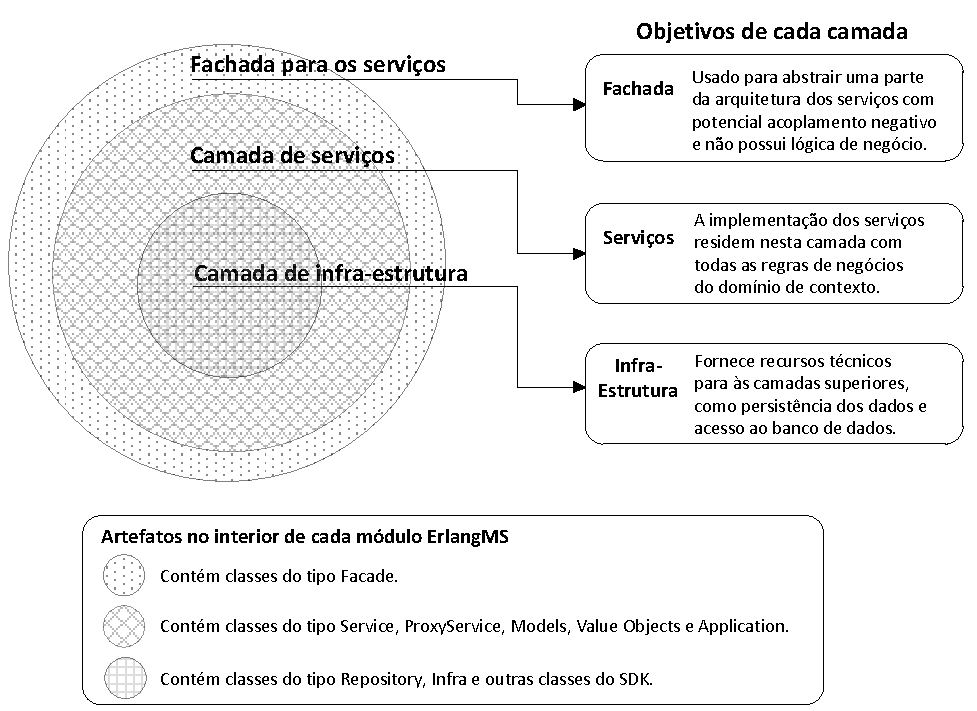
\includegraphics[scale=0.9]{img/processo/arquitetura_modulo.pdf}
\caption{Anatomia de um módulo da camada de serviços.}
\label{fig:arquitetura_modulo}
\end{figure}



\section{Finalidade de cada camada}

Com base nestes aspectos, apresenta-se a seguir uma 
breve descrição da finalidade de cada camada,
no modelo de arquitetura proposto para 
os módulos de serviços.

\subsection{Primeira Camada: De fachada}
	
	Implementa 
	o padrão \emph{ServiceFacade} 
	identificado em~\cite{SOA_patterns_2012}.
	Salienta-se que esta camada não deve 
	conter	lógica de negócio e 
	o seu objetivo é evitar 
	um possível acoplamento indesejado
	ao impedir que a lógica de negócio 
	localizada na camada de serviços
	seja exposta diretamente ao barramento.
	Assim, quando o cliente requisita um 
	serviço ao barramento,
	na verdade, é invocado um 
	método da fachada.

	Em termos práticos, a finalidade
	desta camada é possibilitar que 
	os parâmetros da requisição \acrshort{REST}
	sejam lidos e o método do serviço correspondente seja invocado
	com os dados que ele necessita. E, 
	no caso do serviço retornar
	uma resposta ao cliente, a fachada pode 
	realizar algum 
	processamento opcional (no estudo de caso não foi necessário)
	ou simplesmente retornar o 
	resultado ao cliente\footnote{O
	desenvolvedor não precisa preocupar-se 
	com a transformação dos dados de/e para \acrshort{JSON}, 
	isso é de responsabilidade do \acrshort{SDK} e do barramento.}.

	O Código~\ref{fig:exemplo_fachada} mostra um exemplo
	de fachada para o serviço \emph{QuestionarioService}
	do módulo unb\_questionario,
	onde há três métodos declarados que ao serem
	invocados, ocorrem os 
	seguintes eventos nessa ordem: 
	os dados da requisição
	são lidos a partir do \emph{IEmsRequest request}
	(interface que contém os dados da requisição); 
	após, é obtido a referência ao objeto \emph{QuestionarioApplication}, 
	responsável pelo acesso a camada de serviços do módulo; depois,
	a referência para o objeto do serviço correspondente é recuperada, 
	e finalmente; o método do serviço solicitado é invocado
	com os parâmetros requeridos.
	
	 
	
	
\lstset{language=Java,
        basicstyle=\footnotesize,
        numbers=left,
        numberstyle=\footnotesize,
        tabsize=2,
        numbers=none,
        rulesepcolor=\color{blue}}
             
\renewcommand{\lstlistingname}{Código}             
\begin{lstlisting}[caption=Exemplo de fachada para o serviço QuestionarioService., label=fig:exemplo_fachada] 

package br.unb.questionario.facade;

import br.unb.questionario.service.QuestionarioApplication;

public class QuestionarioFacade extends EmsServiceFacade {
	public Questionario findById(IEmsRequest request){
		Integer id = request.getParamAsInt("id");
		return QuestionarioApplication.getInstance()
			.getQuestionarioService()
			.findById(id);
	}
	
	public Questionario insert(IEmsRequest request){
		Questionario questionario = (Questionario) request.getObject(Questionario.class);
		return QuestionarioApplication.getInstance()
			.getQuestionarioService()
			.insert(questionario);
	}
	
	public boolean vinculaPerguntaAoQuestionario(IEmsRequest request){
		int questionario_id = request.getParamAsInt("id");
		int pergunta_id = request.getPropertyAsInt("pergunta");
		QuestionarioApplication.getInstance()
			.getQuestionarioService()
			.vinculaPerguntaAoQuestionario(questionario_id, pergunta_id);
		return true;
	}
	// outros métodos omitidos...
}
\end{lstlisting}
	
	
\subsection{Segunda Camada: De serviços}	
	
	A camada de serviços consiste na parte mais 
	importante da arquitetura mostrada na Figura~\ref{fig:arquitetura_modulo}, 
	pois na visão de~\cite{evans2004domain, fowler2002patterns},
	é o local onde	concentra-se a lógica de domínio do negócio do sistema.
	Por conta disso, convém destacar que parte
	do foco do \acrshort{DDD},
	como identificado em~\cite{evans2004domain, fowler2002patterns}, 
	situa-se nessa camada, razão pela qual
	o design da arquitetura proposta
	tenta (na medida do possível) 
	não focar em tecnologia, 
	mas, em vez disso, entender as regras do negócio e
	como refleti-las no código fonte da aplicação 
	de maneira agnóstica.

	Nesse sentido, ao modelar a camada de serviços, 
	pode-se fazer uso de diversos \emph{blocos 
	de construção} definidos no \acrshort{DDD},
	que são, essencialmente, os artefatos que constituem
	esta camada. Para exemplificar e explicar 
	alguns conceitos desses artefatos, 
	segue uma descrição
	dos principais elementos utilizados na camada de serviços 
	dos módulos desenvolvidos no \acrshort{SAE}. 
	
	\begin{itemize}
	
		\item Entidades. São as classes de objetos que possuem 
						 identidade, comportamentos (ou métodos) 
						 e um ciclo de vida~\cite{evans2004domain}.
						 Por exemplo, 
						 um aluno do \acrshort{SAE}
						 que se autentica no sistema e realiza
						 a avaliação socioeconômica. Em sistemas Java 
						 típicos, como os desenvolvidos pelo CPD/UnB,
						 as classes de entidades podem 
						 ser comparados a classes \acrfull{POJO}, 
						 embora	um \acrshort{POJO} siga
						 algumas definições de design
						 que uma Entidade não precisa
						 (por exemplo,	ter um construtor padrão
						 sem argumentos e 
						 métodos \textit{getters} e \textit{setters}
						 para os atributos), 			 
						 de acordo com~\cite{kalin2013java}.


		\item \acrfull{VO}. São as classes de objetos
						que são modeladas geralmente para 
						carregar dados e
						possuem o sufixo \emph{Vo}
						no \acrshort{SAE} por convenção.
						Uma classe desse tipo é o
						\emph{CampusVo} que
						possui apenas dois atributos (id e nome)
						e foi implementada para que os serviços 
						do módulo unb\_sae possam carregar a 
						lista de campus a partir de um serviço
						que está no módulo unb\_sitab. Existem
						outras características sobre \acrshort{VO}
						que não serão tratadas aqui por simplicidade
						mas em~\cite{fowler2002patterns} 
						é discutido em mais detalhes.
						
						

		\item \textit{Factory}. São as classes responsáveis
			por \emph{fabricar} os objetos e usadas
			na fabricação dos serviços nessa camada. 
			Essas classes tem 
			o sufixo \emph{Application} por convenção 
			(QuestionarioApplication, por exemplo)
			e apenas por curiosidade, classes desse tipo
			são também conhecidas pelo padrão
			\textit{ApplicationService} no guia de padrões
			de design Java EE (Core J2EE
			Patterns)~\cite{alur2003core}.
			
			Como é possível
			observar no Código~\ref{fig:exemplo_fachada} de exemplo,
			a fachada somente acessa um objeto de
			serviço mediante o QuestionarioApplication. 
			O principal motivo
			para o uso desse design
			no \acrshort{SAE} é esconder 
			a forma como se criam ou
			injetam os objetos (com injeção de dependência),
			uma vez que é desejável que o \acrshort{SDK}
			em outras linguagens de programação
			façam o mesmo,
			independente da tecnologia empregada para isso.
			Outro motivo importante é minimizar
			as dependências e o acoplamento entre os objetos. 
			Note que isso foi obtido, pois,
			é possível verificar que os métodos 
			da fachada acessam somente a interface 
			do serviço e não precisam importar 
			a classe de implementação do serviço,
			somente a classe QuestionarioApplication
			em br.unb.questionario.service.
		
		\item \textit{Services}. São as classes que contém 
				as regras de negócios da aplicação e
				a implementação do serviço
				de acordo com a sua especificação 
				no catálogo de serviços do projeto.
				Note que os objetos do tipo Entidades
				também contém regras de negócios
				porque o \acrshort{DDD} trabalha com objetos 
				com comportamentos 
				e não somente atributos (ou seja, objetivos não anêmicos).
				
				Além disso, uma observação importante
				sobre os serviços identificado em~\cite{fielding1999rfc},
				é que as classes de serviço não devem ter estado,
				obedecendo dessa forma, a restrição REST \textit{Stateless},
				discutida no Capítulo~\ref{fundamentos}.
	\end{itemize}
	
	Para finalizar a descrição dos conceitos discutidos 
	sobre a camada de serviços da arquitetura proposta,	
	o Código~\ref{fig:exemplo_servico} mostra a implementação 
	parcial do código fonte da classe do 
	serviço QuestionarioService com os 3 métodos invocados
	pela fachada demonstrada anteriormente 
	no Código~\ref{fig:exemplo_fachada}. Perceba que 
	o serviço faz uso da camada de infraestrutura apresentada a seguir.
	
	
\lstset{language=Java,
        basicstyle=\footnotesize,
        numbers=left,
        numberstyle=\footnotesize,
        tabsize=2,
        numbers=none,
        rulesepcolor=\color{blue}}
             
\renewcommand{\lstlistingname}{Código}             
\begin{lstlisting}[caption=Exemplo de implementação do serviço QuestionarioService., label=fig:exemplo_servico]

package br.unb.questionario.service;

// imports omitidos para facilitar a visualização

public class QuestionarioService {
	public Questionario findById(Integer id) {
		return QuestionarioInfra.getInstance()
			.getQuestionarioRepository()
			.findById(id);
	}
	
	public Questionario insert(Questionario questionario) {
		questionario.validar();
		return QuestionarioInfra.getInstance()
			.getQuestionarioRepository()
			.insert(questionario);
	}	
	
	public void vinculaPerguntaAoQuestionario(
		int questionario_id, int pergunta_id) {
		Questionario questionario = findById(questionario_id);
		Pergunta pergunta = QuestionarioApplication.getInstance()
								.getPerguntaService()
								.findById(pergunta_id);
		questionario.vinculaPergunta(pergunta);
	}	
	// outros métodos omitidos...
}
\end{lstlisting}
	

\subsection{Terceira Camada: Infraestrutura}	


		É muito comum, parte do software 
		não estar diretamente relacionado 
		ao domínio do negócio, 
		mas a sua infraestrutura de apoio~\cite{avram2007domain}.
		Assim, a finalidade desta camada
		é prover os recursos técnicos
		necessários para as
		camadas superiores do módulo, 
		como o acesso, a persistência
		e a consulta dos objetos em um banco de dados, 
		a escrita de logs para o registro de eventos relevantes,	
		entre outros recursos.

		No entanto,~\cite{evans2004domain, fowler2002patterns} 
		afirmam que esta camada 
		deve prover os recursos 
		tecnológicos de forma isolada,
		não expondo
		os detalhes internos da 
		infraestrutura,
		pois podem comprometer a 
		camada de serviços
		com aspectos
		técnicos do software misturados com
		as regras de negócios. 
		Nesse caso,~\cite{avram2007domain} 
		sugere que a camada de infraestrutura
		seja exposta através de interfaces simples.
	

		Assim como na camada de serviços,
		existem alguns artefatos
		para modelar esta camada, 
		previstos no \acrshort{DDD}~\cite{evans2004domain}.
		Na arquitetura proposta, 
		sugere-se utilizar
		os artefatos \textit{Repository} (Repositório)
	 	e o \textit{Factory}, para lidar
	 	com os desafios discutidos anteriormente.
		Segue uma breve descrição
		de alguns conceitos desses artefatos 
		com exemplos de utilização em código Java.
			
		\begin{itemize}
		
			\item \textit{Repository}.	Tradicionalmente, a maioria das aplicações
			precisam persistir ou recuperar os objetos 
			em algum banco de dados.
			Sendo assim, o objetivo das 	
			classes \textit{Repository} é
			basicamente gerenciar o ciclo de vida dos objetos, 
			como as Entidades ou \acrshort{VO},
			centralizando as 
			operações de criação, modificação, exclusão
			e consulta de objetos em um banco de dados~\cite{vernon2013implementing}.
			
			Para exemplificar,
			o Código~\ref{fig:exemplo_repository} mostra
			a classe de repositório \emph{OcorrenciaRepository} 
			do módulo \emph{unb\_sae}, 
			cujo objetivo é gerenciar o ciclo de vida das
			ocorrências de um estudante, 
			um tipo
			de evento ocorrido em um determinado período	 
			que pode acarretar na suspensão do
			auxílio alimentação,
			mediante justificativa, de acordo 
			com as normas do \acrfull{PNAES}. 
			As classes \textit{Repository}
			na arquitetura proposta possuem
			o sufixo Repository por convenção. 
			
			A primeira observação 
			nessa classe é quanto 
			a sua interface. 
			Por motivos já discutidos,
			as classes \textit{Repository}
			foram projetadas para
			terem uma interface simples. 
			Note que
			a classe OcorrenciaRepository 
			herda de 
			\textit{EmsRepository} (veja a Figura~\ref{fig:diagrama_classe_ems_repository})
			fornecido pelo \acrshort{SDK}
			e não precisa implementar nenhum 
			método público nesse exemplo, 
			uma vez que as operações 
			herdadas são suficientes. Em outras classes,
			poderá ser necessária a criação
			de outros métodos públicos conforme 
			a necessidade. Pode-se notar também
			alguns métodos protegidos
			e que na implementação em Java do \acrshort{SDK}, 
			os repositórios usam o \acrfull{JPA},
			um \textit{framework} de persistência de dados.
			Este é um detalhe técnico que importa
			somente aos repositórios e não devem 
			ser expostos, como 
			verificou-se em~\cite{evans2004domain, fowler2002patterns}.			
			Por curiosidade, o diagrama de classe 
			na Figura~\ref{fig:diagrama_classe_ems_repository}
			exibe as operações comuns a todas
			as classes \textit{Repository}
			na arquitetura.
		
		
\begin{figure}[htb]
\centering
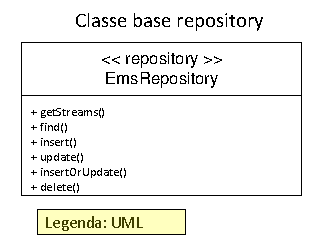
\includegraphics[scale=1.5]{img/processo/exemplo_classe_repository.pdf}
\caption{Classe base repository.}
\label{fig:diagrama_classe_ems_repository}
\end{figure}
\FloatBarrier
	
	

	


			Como pode-se ver na Figura~\ref{fig:diagrama_classe_ems_repository},
			há uma operação denominada \textit{getStreams()}, 
			que	merece uma explicação. A ideia
			desse método surgiu 
			no estudo de caso (não fazia parte 
			da proposta inicial da arquitetura) 
			para
			fornecer uma 
			interface comum para 
			consulta de objetos.
			Ou seja,
			como a maioria das operações 
			geralmente são consultas (nos sistemas do CPD/UnB),
			buscou-se uma forma de expor uma 
			pequena \acrshort{API}
			para que o desenvolvedor não
			precise 
			implementar um novo método 
			de consulta sempre que for 
			necessário 
			pesquisar objetos por 
			determinada 
			condição (contando que a pesquisa seja simples).
			O Código~\ref{fig:exemplo_get_stream} ilustra o uso 
			desta \acrshort{API} em alguns
			métodos da entidade Aluno fazendo uso 
			do método \textit{getStreams()},
			onde é possível notar uma certa praticidade
			com o uso desta funcionalidade,
			além de possibilitar emitir as consultas
			usando uma linguagem tipificada
			em vez de usar as linguagens de consultas
			tradicionais, como a \acrfull{SQL}.
			
		
			\item \textit{Factory}. São as classes responsáveis
			por fabricar os 
			repositórios (ou outros objetos)
			da camada de infraestrutura, 
			tendo por convenção,
			o sufixo \emph{Infra} neste trabalho.
			No Código~\ref{fig:exemplo_get_stream},
			é possível observar 
			que a classe Aluno
			acessa os repositórios requeridos
			por meio da classe \emph{SaeInfra}, 
			o \textit{Factory} da camada de 
			infraestrutura
			do módulo unb\_sae. 
			O principal 
			motivo do uso desse design,
			como discutido anteriormente,
			é esconder a forma como se criam
			os objetos.
		
		\end{itemize}







\lstset{language=Java,
        basicstyle=\footnotesize,
        numbers=left,
        numberstyle=\footnotesize,
        tabsize=2,
        numbers=none,
        rulesepcolor=\color{blue}}
             
\renewcommand{\lstlistingname}{Código}             
\begin{lstlisting}[caption=Exemplo de implementação do repositório QuestionarioRepository., label=fig:exemplo_repository]
package br.unb.sae.infra;

// imports omitidos para facilitar a visualização

public class OcorrenciaRepository extends EmsRepository<Ocorrencia>{
	
	@PersistenceContext(unitName = "service_context")
	protected EntityManager saeContext;
	
	@Override
	protected Class<Ocorrencia> getClassOfModel() {
		return Ocorrencia.class;
	}

	@Override
	protected EntityManager getEntityManager() {
		return saeContext;
	}

}
\end{lstlisting}


\lstset{language=Java,
        basicstyle=\footnotesize,
        numbers=left,
        numberstyle=\footnotesize,
        tabsize=2,
        numbers=none,
        rulesepcolor=\color{blue}}
             
\renewcommand{\lstlistingname}{Código}             
\begin{lstlisting}[caption=Exemplo de uso do método getStream() dos repositórios para consulta., label=fig:exemplo_get_stream]
package br.unb.sae.model;

// imports omitidos para facilitar a visualização

public class Aluno{

	private boolean assinouTermoConcessaoValeAlimentacao(
		String periodo) {
			int this_aluno = getId();
			return SaeInfra.getInstance()
				.getAssinaturaTermoBaRepository()
				.getStreams()
				.anyMatch(a -> a.getAluno() == this_aluno &&
							    a.getPeriodo().equals(periodo));
	}

	private boolean existeOcorrenciaAberto(
		String periodo, Date dataInicio) {
			int this_aluno = getId();
			return SaeInfra.getInstance()
				.getOcorrenciaRepository()
				.getStreams()
				.anyMatch(a -> a.getAluno() == this_aluno &&
							   a.getPeriodo().equals(periodo) &&
					       a.getDataInicio().equals(dataInicio));
	}

	public List<Ocorrencia> getListaOcorrencia() {
		int aluno_id = getId();
		return SaeInfra.getInstance()
				.getOcorrenciaRepository()
				.getStreams()
				.where(a -> a.getAluno() == aluno_id)
				.toList();
	}    
	
	public Ocorrencia findOcorrenciaById(Integer idOcorrencia) {
		return SaeInfra.getInstance()
			.getOcorrenciaRepository()
			.findById(idOcorrencia);
	}
	
	public List<AssinaturaTermoBa> getListaAssinaturaTermoConcessaoValeAlimentacao() {
		int this_aluno = getId();
		return SaeInfra.getInstance()
				.getAssinaturaTermoBaRepository()
				.getStreams()
				.where(a -> a.getAluno() == this_aluno)
				.toList();
	}
	// outros métodos omitidos
}
\end{lstlisting}





